\documentclass[12pt, spanish, oneside, onecolumn, a4paper]{report}
\usepackage[spanish,activeacute]{babel}
\usepackage[latin1,utf8]{inputenc}
\usepackage{times}
\usepackage[T1]{fontenc}
\usefont{T1}{arial}{m}{n}
\oddsidemargin 0in
\textwidth 6.75in
\topmargin 0in
\textheight 8.5in
% \parindent 0em
\parskip 2ex

\usepackage{fancyheadings}
\headheight 35pt
\usepackage{graphicx}
\usepackage[colorlinks=true, urlcolor=blue, filecolor=green,
linkcolor=red, pdfkeywords={}, pagebackref, pdfpagemode=UseOutlines,
bookmarksopen=true]{hyperref}

\usepackage{tabularx} 
\usepackage{colortbl} 
\usepackage{wrapfig} 

\usepackage{tabulary} 
\setlength\tymin{699pt} 
\setlength\tymax{700pt} 
\setlength\doublerulesep{0.5px} 

\graphicspath{{./img/}} 

\usepackage{epic} 
\makeatletter 

\renewcommand{\contentsname}{Indice}
\renewcommand{\appendixname}{Apéndice}
\renewcommand{\figurename}{Figura}
\renewcommand{\listfigurename}{Indice de figuras}
\renewcommand{\tablename}{Tabla}
\renewcommand{\listtablename}{Indice de tablas}

\definecolor{mygray}{gray}{.95} % 
\definecolor{Gray}{gray}{.95} % 
%\colorbox{Gray}{\makebox[\hfill][l]{Title}} 

\DeclareTextFontCommand{\emph}{\bf\em} % 
\DeclareRobustCommand{\em}{
  % 
  \@nomath\em 
  \if b\expandafter\@car\f@series\@nil 
  % 
  \normalfont 
  \else 
  \bfseries 
  \fi
}

\newcommand{\shellcmd}[1]{ %
  \colorbox{Gray}{
    \indent\indent\texttt{\footnotesize\$ #1}
  }
  \colorbox{mygray}{
    \indent\indent\texttt{\textbf{\footnotesize\$} #1}
  }
} 

\newcommand{\rootshellcmd}[1]{
  \colorbox{mygray}{
    \indent\indent\texttt{\textbf{\footnotesize\#} #1}
  } 
  \indent\indent\texttt{\footnotesize\# #1}
} 

\newcommand{\svngit}[2]{% 
  \begin{tabular}{| l | l |} 
    \hline subversion: & git: \\
    \hline 
    \colorbox{mygray}{\texttt{\textbf{\footnotesize\$} #1}} & \colorbox{mygray}{ \texttt{\textbf{\footnotesize\$} #2}} 
  \end{tabular}
  % 
} 
\usepackage[toc,nonumberlist]{glossaries} 
\makeglossaries 

\def\maketitle{% 
  \null 
  \thispagestyle{empty}% 
  \vfill 
  \begin{center}
    \leavevmode 
    \normalfont 
    
\includegraphics{logo.png}%\\[1cm] %
    {\LARGE \@title\par}% 
    \vskip 1cm {\Large \@author\par}% 
    \vskip 1cm {\Large \@date\par}% 
  \end{center}% 
  \vfill 
  \null 
  \cleardoublepage
}

\makeatother 
\usepackage[section]{placeins} 
\begin{document} 
\pagestyle{fancy} 
\lhead{
\includegraphics[width=3cm,keepaspectratio=true]{logo.png} } %

\title{ Git } 
\date{ 
  \today\ } 
\author{ Ing. Anielkis Herrera } 
\pagenumbering{roman} 
\maketitle
\begin{abstract}
  Guía de uso de la herramienta Git para control de versiones 
\end{abstract} 
\newpage 
\pagenumbering{arabic} 
\chapter{Introducción a Git} 
\label{chap:intro} 
\newacronym[longplural=Sistemas de Control de Versiones]{scv}{SCV}{Sistema de Control de Versiones} 

\newacronym[longplural=Sistemas de Control de Versiones Distribuidos]{scvd}{SCVD}{Sistema de Control de Versiones Distribuido} 

\newacronym[longplural=Sistemas de Control de Versiones Centralizados]{scvc}{SCVC}{Sistema de Control de Versiones Centralizado}

\newglossaryentry{Linux}{description={es un término genérico que se refiere a la familia de sistemas operativos ``parecidos a Unix'' que utilizan el núcleo Linux}}

Git es un \gls{scvd}, desarrollado como sistema de software libre y diseñado para manejar desde proyectos pequeños hasta muy grandes, con gran rapidez y eficiencia. Git es fácil de aprender y tiene una huella pequeña en el sistema, con un rendimiento increíblemente rápido. Supera a otros \glspl{scv} como Subversion, CVS, Perforce y ClearCase con características como trabajo con ramas locales, áreas de ``puesta en escena'' muy convenientes, y varios estilos de flujo de trabajo. 

\section{Acerca de Git} 
\label{sec:aboutgit} 
\subsection{Creación y fusión de ramas} 
\label{sec:branchingandmerging} La función de Git que realmente lo hace destacar de entre la mayoría de los \gls{scv} es su modelo de ramificación. Git permite y alienta a tener varias ramas locales que pueden ser completamente independientes una de otra. La creación, fusión y supresión de las líneas de desarrollo toma solo unos instantes de segundo. Esto significa que se pueden hacer cosas como: 
\begin{description} 
\item [Cambio de contexto sin fricción:] crear una rama para probar una idea, adicionar contenido al historial un par de veces, volver a la rama desde donde se ramificó, aplicar un parche, cambiar de nuevo a donde se está experimentando, y fusionar las ramas para adicionar los cambios del experimento a la rama original. 
\item [Líneas de desarrollo separadas en roles:] tener una rama que siempre contiene sólo lo que va a la producción, otra a dónde se fusionan el código en que se ha trabajado, para probarlo, y varios más pequeños para el día a día. 
\item [Función de flujo de base:] crear nuevas ramas para cada nueva característica en que se esté trabajando por lo que perfectamente puede alternar entre ellas, y a continuación eliminar cada rama cuando esta característica se fusione en la línea principal. 
\item [Experimentación desechable:] crear una rama en la que experimentar , darse cuenta de que no va funcionar el experimento, y simplemente eliminarla - el abandono de un trabajo fallido que nadie más va a ver. 
\end{description} 
\begin{wrapfigure}[15]{r}{0.65\textwidth}     % 
  \begin{center} 
    
\includegraphics[width=.6\textwidth,keepaspectratio=true]{branches.png} % 
  \end{center} 
  \caption{Ramas en Git.} 
  \label{otrosvcs} 
\end{wrapfigure} En particular, cuando se ``empuja'' (\emph{\textbf{push}}) a un repositorio remoto, no es necesario hacerlo a todas las ramas. Se puede elegir compartir sólo una de las ramas, unas pocas de ellas o todas ellas. Esto permite probar nuevas idea s sin preocuparse de tener que planificar cómo y cuándo se va a fusionar o compartir las con otros. Como se podrá ver posteriormente, se puede compartir la rama con otro desarrollador, con el que se puede trabajar en esa idea, sin necesidad de adicionarla al repositorio central. Hay maneras de lograr algo de esto con otros sistemas, pero la obra en cuestión es mucho más difícil y propensa a errores. Git hace este proceso muy fácil y esto cambia la forma en la mayoría de los desarrolladores trabajan cuando lo aprenden. 

\subsection{Pequeño y rápido} 
\label{sec:smallandfast} Git es rápido. Con Git, practicasen todas las operaciones son realizadas localmente, dándole una gran ventaja sobre los \gls{scvc} que constantemente tienen que comunicarse con el servidor. Git fue hecho para trabajar con el núcleo Linux, lo que significa que tiene que trabajar eficientemente con repositorios de código muy grandes desde el primer día. Git está escrito en \textbf{C}, reduciendo la carga de ejecución asociada a lenguajes de alto nivel. La velocidad y el rendimiento son algunos de los principios seguidos desde los inicios de su diseño. 

\subsection{Distribuido} 
\label{sec:distributed} Una de las mejores características de cualquier 
\gls{scvd}, Git incluido, es que e s precisamente ``distribuido''. Esto significa que en lugar de hacer un ``checkout'' de la punta actual del código fuente, se hace un ``clon'' de todo el repositorio. 

\subsubsection{Múltiples copias de seguridad} 
\label{sec:multiplebackups} Esto significa que aún si se utiliza un flujo de trabajo centralizado, cada usuario es esencialmente una copia de seguridad del servidor principal. Cada una de es tas copias puede ser utilizada para sustituir el servidor central en caso de fallo o corrupción. En efecto, no hay un solo punto de fallo utilizando Git, a no ser que sólo se use una copia del repositorio. 
\clearpage 
\subsubsection{Cualquier flujo de trabajo} 
\label{sec:anyworkflow} Debido a la naturaleza distribuida de Git y un magnífico sistema de ramificación, un número casi infinito de flujos de trabajo se puede implementar con relativa facilidad. 
\paragraph{Flujo de trabajo estilo Subversion:} 
\begin{wrapfigure}{r}{0.65\textwidth} 
  \begin{center} 
    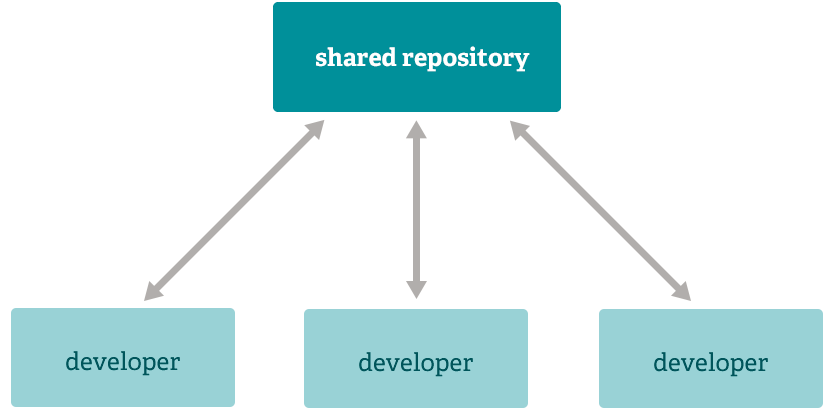
\includegraphics[width=.6\textwidth,keepaspectratio=true]{workflow-a.png} 
  \end{center} 
  \caption{Modelo centralizado estilo Subversion.} 
\end{wrapfigure} Un flujo de trabajo centralizado es bastante común, especialmente para personas cambiando desde sistemas centralizados. Git no permite que se ``empuje''(hacer \textbf{\emph{push}}) al servidor si alguien lo ha hecho desde la última vez que se descargó de él, por lo que un modelo centralizado donde todos los desarrolladores hacen \textbf{\emph{push}} al mismo servidor funciona bien. 
\paragraph{Flujo con gerente integrador:} 
\begin{wrapfigure}{r}{0.65\textwidth} 
  \begin{center} 
    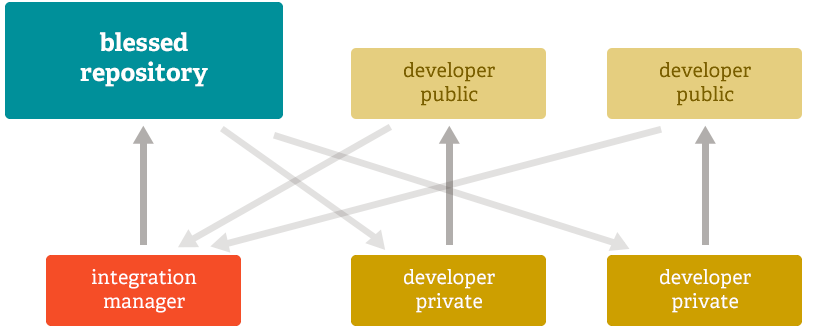
\includegraphics[width=.6\textwidth,keepaspectratio=true]{workflow-b.png} 
  \end{center} 
  \caption{Modelo con gerente integrador.} 
\end{wrapfigure} Otro flujo de trabajo, común en Git, consiste en un gestor de integración - una sola persona que es quien puede adicionar al repositorio ``bendecido''(el \emph{repositorio principal del sistema}). Un número de desarrolladores luego de clonar ese repositorio, empujan a sus propios repositorios independientes , y piden al integrador que revise y fusione sus cambios a ese repositorio. Este es el tipo de modelo de desarrollo visto a menudo con software libre o repositorios en \textbf{Github}. 
\paragraph{Flujo basado en un dictador y sus lugartenientes:} 
\begin{wrapfigure}{r}{0.65\textwidth} 
  \begin{center} 
    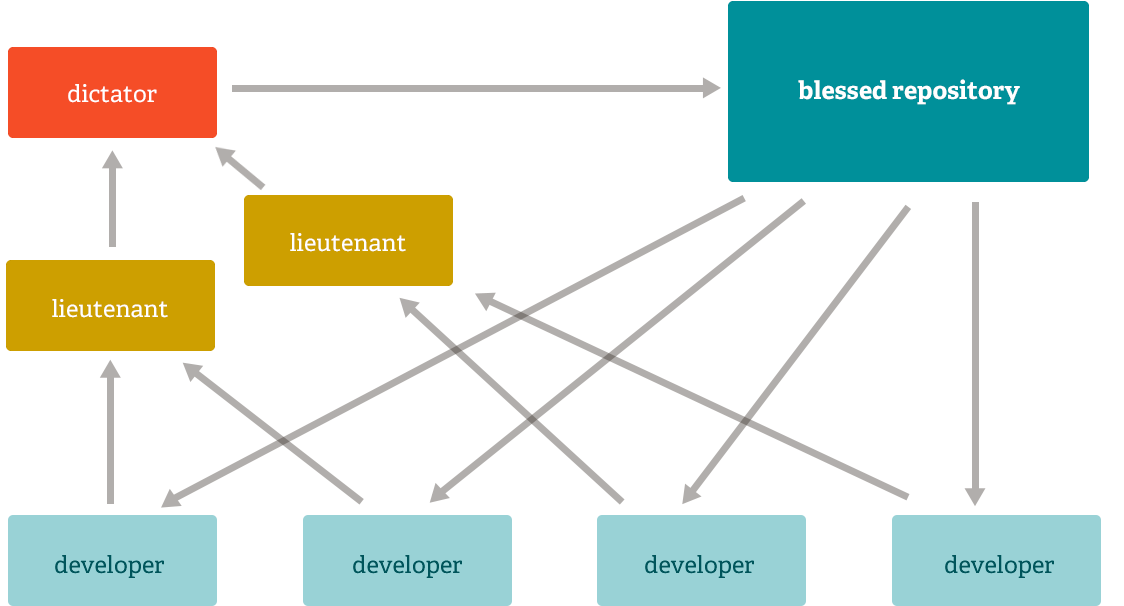
\includegraphics[width=.6\textwidth,keepaspectratio=true]{workflow-c.png} 
  \end{center} 
  \caption{Modelo con dictador y lugartenientes.} 
\end{wrapfigure} Para proyectos más grandes, un flujo de trabajo de desarrollo como el del núcleo Linux es a menudo eficaz. En este modelo, algunas personas ( ``lugartenientes'' ) están a cargo de un subsistema específico del proyecto y fusionan todos los cambios relacionados con ese subsistema. Otra integrador (el ``dictador'' ) puede extraer los cambios sólo de sus lugartenientes (luego que estos los revisaron e integraron a sus subsistemas) y luego empujar al repositorio ``bendecido'' de dónde todo el mundo usa para trabajar. 
\clearpage 
\subsection{Seguridad de los datos} 
\label{sec:dataassurance} El modelo de datos que usa Git garantiza la integridad criptográfica de cada parte de su proyecto. A cada archivo y revisión en el historial se le realiza una suma de comprobación (suma de chequeo) y es recuperado por medio de su suma de chequeo al recrear el directorio. Por esto es imposible sacar nada de Git que no sean los bits exactos que se le ponen dentro. 
\begin{wrapfigure}{r}{0.65\textwidth} 
  \begin{center} 
    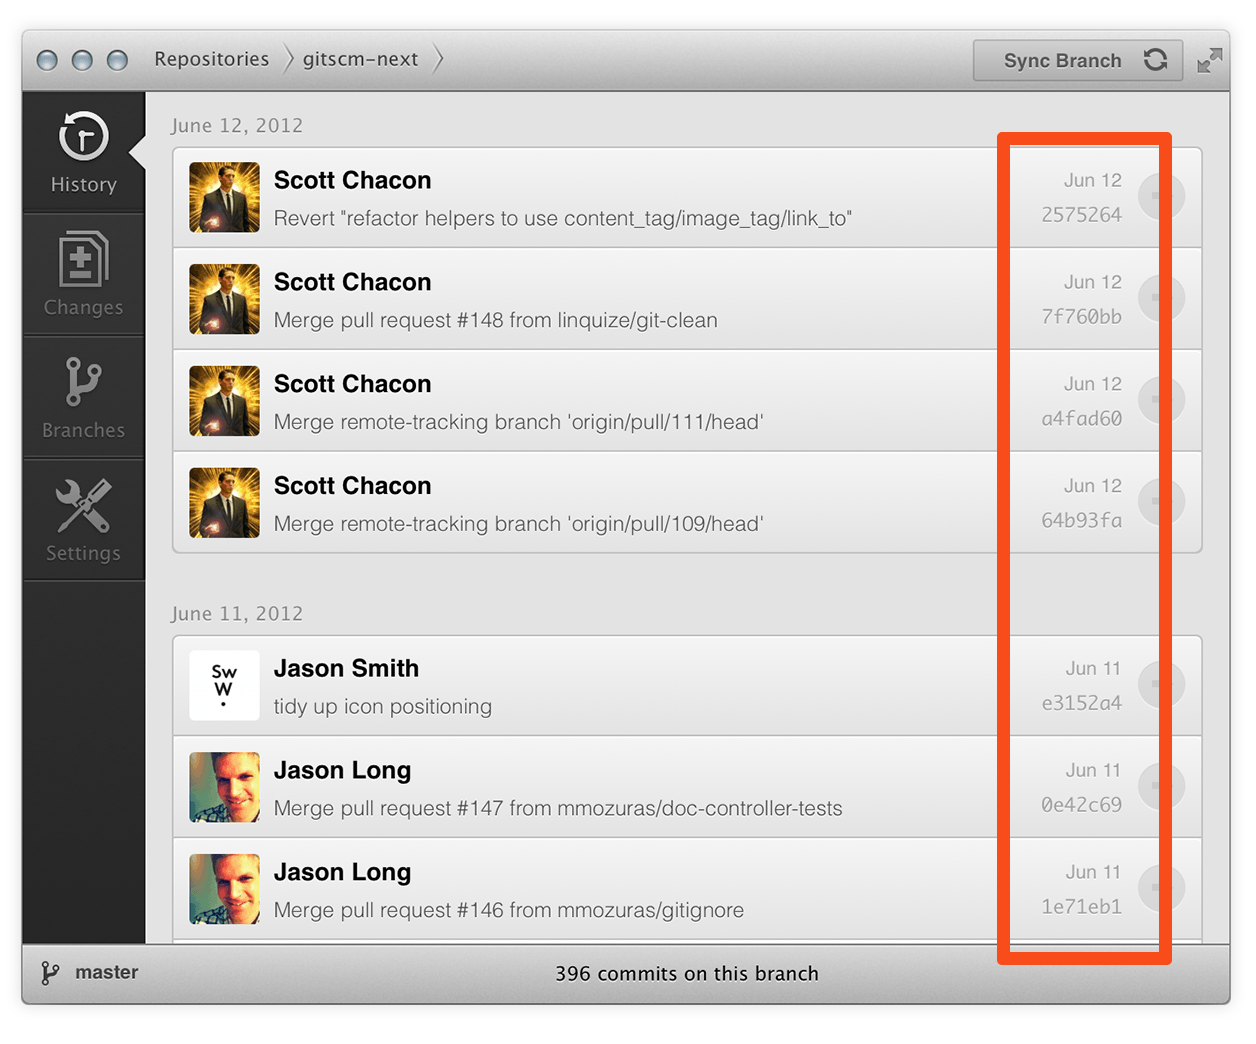
\includegraphics[width=.6\textwidth,keepaspectratio=true]{assurance.png} 
  \end{center} 
  \caption{Sumas de chequeo.} 
\end{wrapfigure} También es imposible cambiar cualquier archivo, la fecha, el mensaje con que se adicionó al historial, o cualquier otro dato en un repositorio Git sin cambiar los identificadores de todo lo que ocurrió después de adicionarlo. Esto significa que si usted tiene un ID de un ``\textbf{commit}'' (una revisión), puede estar seguro no sólo de que el proyecto es exactamente el mismo que cuando se adicionó, sino que nada en su historial cambió. La mayoría de los 
\gls{scvc} no proveen esta integridad de forma predeterminada. 
\clearpage 
\subsection{Zona de espera} 
\label{sec:stagingarea} 
\begin{wrapfigure}{r}{0.65\textwidth} 
  \begin{center} 
    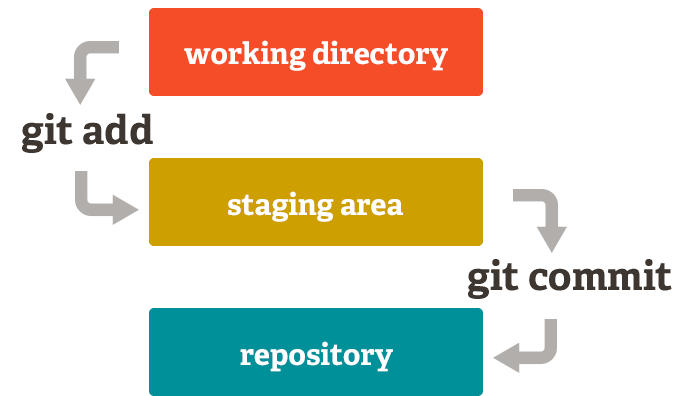
\includegraphics[width=.6\textwidth,keepaspectratio=true]{index1.png} 
  \end{center} 
  \caption{Zona de espera.} 
\end{wrapfigure} A diferencia de los otros sistemas, Git tiene algo que se llama la ``zona de espera'' o ``índice''. Esta es una zona intermedia en la que los 
\textbf{\emph{commit s}} pueden ser formateados y o revisados antes de terminar de adicionarlos como una revisión en el historial. Una cosa que distingue a Git de otras herramientas es que es posible para organizar rápidamente las modificaciones en los archivos, sin adicionar todas las modificaciones hechas en una sola revisión en el historial. 
\begin{wrapfigure}{r}{0.65\textwidth} 
  \begin{center} 
    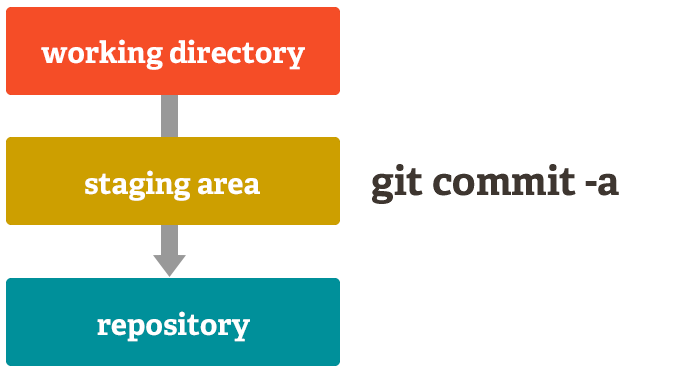
\includegraphics[width=.6\textwidth,keepaspectratio=true]{index2.png} 
  \end{center} 
  \caption{Zona de espera.} 
\end{wrapfigure} Esto le permite poner en escena sólo partes de un archivo modificado. Atrás han quedado los días de hacer dos modificaciones lógicamente no relacionadas en uno o varios archivos, antes de darse cuenta de que se ha olvidado adicionar una de ellas al historial. Ahora se puede incluir sólo uno de cambios realizados al archivo, en u na revisión y luego adicionar otro cambio en otra revisión. Esta función se puede utilizar para múltiples cambios, según sea necesario, permitiendo organizar mejor los cambios adicionados, por ejemplo, según funcionalidad o módulo. Por supuesto, Git también puede olvidar esta funcionalidad si no se desea este tipo de control, sólo adicionando ``$-$a'' al comando, adiciona 
\textbf{TODOS} los cambios realizados a los archivos conocidos por Git (todos los que han sido adicionados al historial en la revisión anterior); haciendo que Git se comporte como Subversion al realizar un 
\textbf{commit}. 
\chapter{Comenzando con Git} 
\label{chap:gettingstarted} 
\section{Lo esencial de Git} 
\label{sec:gitbasics} Entonces, ¿qué es Git en pocas palabras? Esta es una sección importante de absorber, porque si se entiende lo que es Git y los fundamentos de cómo funciona, podrá utilizar Git de una forma más eficaz y probablemente será mucho más fácil. A medida que se aprenda Git, se debe intentar limpiar la mente de las cosas que se pueden conocer de otros 
\gls{scv}, tales como Subversion y Perforce , lo cual ayudará a evitar confusiones sutiles cuando se utiliza la herramienta. Git almacena información y piensa en forma muy diferente a los otros sistemas, a pesar de que la interfaz de usuario es bastante similar; entender esas diferencias ayudará a evitar que se vuelva confuso mientras se esté utilizando. 
\subsection{Imágenes del contenido, no las diferencias} 
\label{sec:snapshotsnotdifferences} 
\begin{wrapfigure}[15]{r}{0.65\textwidth} % 
  \begin{center} 
    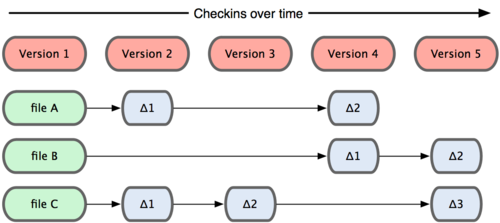
\includegraphics[width=.6\textwidth,keepaspectratio=true]{18333fig0104-tn.png} % 
  \end{center} 
  \caption{Otros sistemas tienden a almacenar datos como cambios a una versión base de cada archivo.} 
  \label{otrosvcs} 
\end{wrapfigure} La principal diferencia entre Git y cualquier otro 
\gls{scv} (Subversion y amigo s incluidos) es la forma en Git piensa en sus datos. Conceptualmente, la mayoría d e los otros sistemas almacena información como una lista de los cambios basados en ficheros. Estos sistemas (CVS, Subversion, Perforce, Bazaar, y así sucesivamente ) piensan en la información que almacenan como un conjunto de archivos y los cambios hechos a cada fichero en el tiempo, como se ilustra en la Figure~\ref{otrosvcs}. 

\begin{wrapfigure}{r}{0.65\textwidth} 
  \begin{center} 
    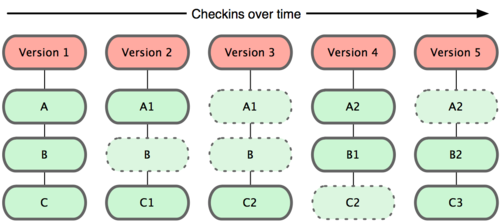
\includegraphics[width=.6\textwidth,keepaspectratio=true]{18333fig0105-tn.png} 
  \end{center} 
  \caption{Git almacena los datos como imágenes del proyecto a través del tiempo.} 
  \label{gitsnapshot} 
\end{wrapfigure}

Git no piensa ni almacene sus datos de esta forma. En su lugar, Git modela sus datos más como un conjunto de instantáneas de un pequeño sistema de archivos. Cada vez que se adiciona, o guarda el estado de el proyecto en Git, básicamente se toma una fotografía de sus archivos en ese momento y almacena una referencia a esa instantánea. Para ser eficaz, si los archivos no se han modificado, Git no almacena el archivo de nuevo, sólo un enlace al archivo anterior idéntico que ya ha almacenado. Git modela sus datos más como en la Figura 
\href{gitsnapshot}. Esta es una distinción importante entre Git y casi todos los otros 
\gls{scv}. Hace que Git reconsidere casi todos los aspectos de control de versiones que la mayoría de los otros sistemas de copiado de la generación anterior. Esto hace que Git más como un pequeño sistema de archivos con algunas herramientas increíblemente poderosas construidas en la parte superior de la misma, en lugar de simplemente un 
\gls{scv}. Se verán algunos de los beneficios que obtiene al pensar en sus datos de esta manera cuando se vea la ramificación en Git. 
\subsection{Casi cada operación es local} 
\label{sec:nearlyoperationlocal} La mayoría de las operaciones en Git sólo necesitan archivos y recursos locales para operar - por lo general no se necesita información desde otro ordenador de la red . Si estás acostumbrado a un \gls{scvc} donde la mayoría de las operaciones tienen esa sobrecarga de latencia de la red, este aspecto de Git te hará pensar que ``los dioses de la velocidad han bendecido Git con poderes no terrenales''. Porque tienes toda la historia del proyecto ahí mismo en el disco local, la mayoría de las operaciones parecen casi instantánea. Por ejemplo, para navegar por la historia del proyecto, Git no necesita salir al servidor para obtener la historia y mostrarla, sino que simplemente se lee directamente de la base de datos local. Esto significa que se verá la historia del proyecto casi al instante. Si se desea ver los cambios introducidos entre la versión actual de un archivo y el archivo de hace un mes, Git puede buscar el archivo hace un mes y hacer un cálculo de la diferencia local, en lugar de tener que pedirle a un servidor remoto la información de una versión anterior del archivo, para calcularlo localmente. Esto también significa que hay muy poco que no se pueda hacer si se está desconectad o de la red o de la VPN. Si se está en un avión, o en un tren y se quiere hacer un poco de trabajo, se puede ir haciendo modificaciones, y al llegar la una conexión d e red que se desea se ``descargan'' los cambios nuevos del servidor y ``suben'' los cambios realizados localmente. Si se va a casa y no logra que funcione bien el cliente VPN, usted todavía puede trabajar. En muchos otros sistemas, hacerlo así que es imposible o doloroso. En Perforce, por ejemplo , no se puede hacer mucho cuando no se está conectado al servidor, y en Subversion y CVS, se puede editar lo s archivos, pero no puede confirmar (hacer ``commit'') los cambios a la base de datos (ya que su base de datos está sin conexión, en el servidor). Esto puede no parecer un gran problema, pero puede que se sorprenda la gran diferencia que puede representar. 
\subsection{Git tiene integridad} 
\label{sec:githasintegrity} A todo en Git, se le realiza una suma de chequeo (\emph{checksum}) y es referenciado por esa suma de chequeo. Esto significa que es imposible cambiar el contenido de un archivo o directorio sin que Git lo note. Esta funcionalidad está incluida en Git en los más bajos niveles y es parte integral de su filosofía. Por esto no s e puede perder la información en tránsito o que se produzca una corrupción de los archivos sin que Git sea capaz de detectarlo. El mecanismo que usa Git para esta suma de comprobación se llama \emph{\textbf{hash SHA-1}}. Es una cadena de 40 caracteres, compuesta de números hexadecimales (del 0 al 9 y de A a la F) y es calculada en base al contenido de un archivo o directorio en Git. Un ``\emph{hash SHA-1}'' se algo como esto: 

\textbf{24b9da6552252987aa493b52f8696cd6d3b00373} Se verán estos valores hash por todos lados en Git, ya que los usa mucho. De hecho , Git almacena todo no por nombre de archivo, sino utilizando el valor hash de s u contenido en la base de datos de Git.

\subsection{Git generalmente sólo añade datos} 
\label{sec:Gitonlyaddsdata}

Cuando se realizan acciones en Git, casi todas ellas sólo añaden datos a la base de datos de Git. Es muy difícil hacer que el sistema realice una operación que no se pueda deshacer o que borre información de alguna forma. Al igual que en cualquier 
\gls{scv}, se pueden perder o estropear los cambios que no se hayan adicionado a Git aún (que no se le haya hecho ``commit''), pero después de haberle hecho \emph{commit} a unos cambios, es muy difícil de que esa información no se pueda recuperar, aún más difícil si se utiliza algún servidor remoto. Llevándolo aún más lejos, cuando una revisión (un \emph{commit}) se deshace, es quitado del historial, Git no lo borra, sino que se puede recuperar mientras no se realice una ``limpieza en profundidad''. Esto permite que se pueda experimentar libremente, sin temor a realizar un daño severo al proyecto. 

\subsection{Los tres estados} 
\label{sec:threestates} Esta es la cosa más importante a recordar acerca de Git si se quieres que el resto de su proceso de aprendizaje fluya sin problemas. Git tiene tres estados principales en que los archivos pueden residir en: 
\textbf{commited} (comprometido), 
\ textbf{modified} (modificado) y 
\textbf{staged} (puesta en escena). 
\textbf{Commited} significa que los datos se almacenan de forma segura en su base de datos local. 
\textbf{Modified} significa que se ha modificado el archivo pero no lo ha hecho 
\textbf{commit} a su base de datos todavía. Y 
\textbf{staged} significa que se ha marcado un archivo modificado en su versión actual para entrar en tu próxima confirmación instantánea (próximo 
\emph{commit}). 
\begin{wrapfigure}[18]{r}{0.52\textwidth} 
  \begin{center} 
    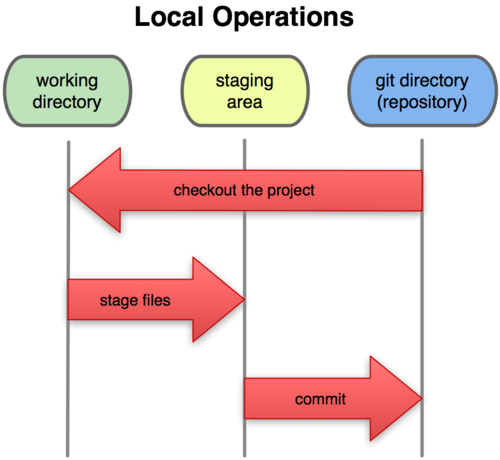
\includegraphics[width=.45\textwidth,keepaspectratio=true]{18333fig0106-tn.png} 
  \end{center} 
  \caption{Directorio de trabajo, área de preparación y directorio Git.} 
  \label{gitsnapshot} 
\end{wrapfigure} Esto nos lleva a 3 secciones principales en un proyecto Git: 
\begin{description} 
\item [el 
  \emph{directorio Git}:] es el 
  \emph{repositorio local} de Git donde se almacenan los metadatos y la base de datos de objetos del proyecto. Esta es la parte más importante de Git, y es lo que se copia cuando se clona un repositorio desde otro equipo. 
\item [el 
  \emph{directorio de trabajo}:] es donde se encuentran los archivos de una revisión para trabajar. Estos archivos se extraen de la base de datos comprimida en el directorio Git y se coloca en el disco para que se puedan utilizar o modificar. 
\item [el 
  \emph{área de preparación}:] también llamada 
  \emph{área intermedia}, 
  \emph{área de caché} o de 
  \emph{puesta en escena} (\textbf{staging area}) es un archivo simple, generalmente dentro del directorio Git, que almacena información acerca de lo que se hará en el próximo 
  \textbf{commit}. A veces se le llama ``\emph{índice}'', pero se está convirtiendo en estándar para referirse a él como el 
  \emph{área de preparación}. 
\end{description} Un flujo básico utilizando Git es algo como esto: 
\begin{enumerate} 
\item Se modifican los archivos en el 
  \emph{directorio de trabajo}. 
\item Se organizan los archivos o modificaciones dentro de éstos que se desean adicionar, y pasándolos al 
  \emph{área de preparación}.

\item Se hace un 
  \textbf{commit}, que toma los archivos como están en el 
  \emph{área de preparación} y almacena una instantánea permanentemente en el directorio Git, integrándola a la historia del proyecto. 
\end{enumerate} Si una versión concreta de un archivo está en el directorio de Git, se considera 
\emph{commited}. Si se ha modificado, pero se ha añadido al área de preparación, está 
\emph {staged}. Y si se ha sido modificado desde que fue extraído de Git y no se pasó al área de preparación, está ``modified''. 

\section{Instalando Git} 
\label{sec:installgit} 

\subsection{Linux} 
\label{sec:installlinux} Si se instará Git a través de paquetes binarios de las distribuciones, esto se realizará como con cualquier otro software: 
\rootshellcmd{yum install git-core} 
\rootshellcmd{apt-get install git} o 
\rootshellcmd{aptitude install git} 

\subsection{MacOSX} 
\label{sec:installmac}

Hay dos maneras fáciles de instalar Git en un Mac. La forma más fácil es usar el instalador gráfico de Git, que se puede descargar desde la página de Google Code: 
\begin{verbatim*} http://code.google.com/p/git-osx-installer 
\end{verbatim*} 
\begin{wrapfigure}{r}{0.65\textwidth} 
  \begin{center} 
    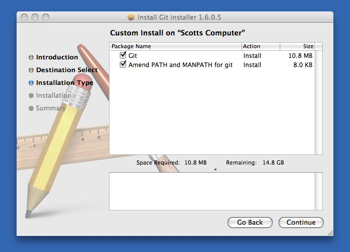
\includegraphics[width=.6\textwidth,keepaspectratio=true]{18333fig0107-tn.png} 
  \end{center} 
  \caption{ Instalador de Git para OS X.} 
\end{wrapfigure} 
\clearpage

La otra gran manera es instalar Git a través de MacPorts ( \url{http://www.macport s.org} ). Si tienes MacPorts instalado, instalar Git a través de: 

\shellcmd{sudo port install git-core +svn +doc +bash\_completion +gitweb}

No se tiene que añadir todos los extras, pero es probable que desee incluir svn, y aún más en caso de que se tenga que usar Git con repositorios de Subversion. 

\subsection{Windows} 
\label{sec:installwindows}

Instalar Git en Windows es muy fácil. Simplemente se descarga el archivo ejecutable de instalación desde la página de Git (\url{http://www.git-scm.com/}), y se ejecuta:

\begin{figure}[hb] 
  \begin{center} 
    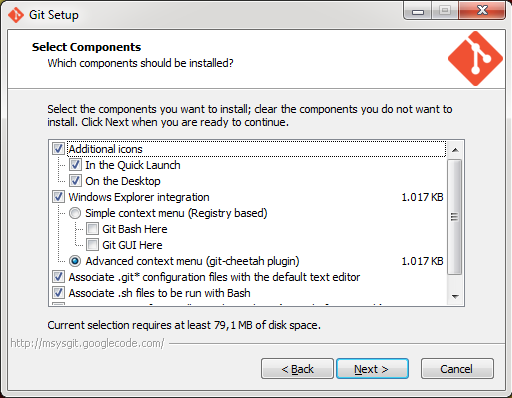
\includegraphics[width=.6\textwidth,keepaspectratio=true]{3.png} 
  \end{center} 
\end{figure} 
\clearpage

Se deben dejar las opciones por defecto: 
\begin{figure}[hb] 
  \begin{center} 
    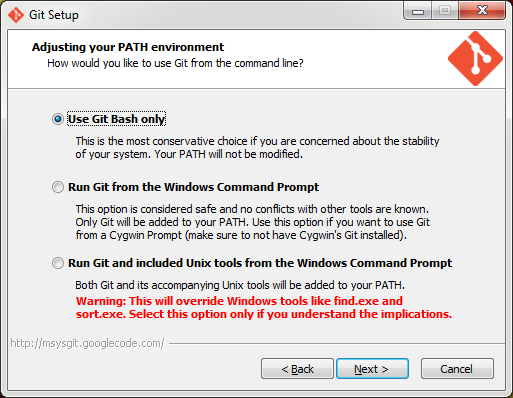
\includegraphics[width=.45\textwidth,keepaspectratio=true]{4.png} 
  \end{center} 
  \caption{Se selecciona interfaz Bash (Unix) para comandos complejos} 
\end{figure} 
\begin{figure}[hb] 
  \begin{center} 
    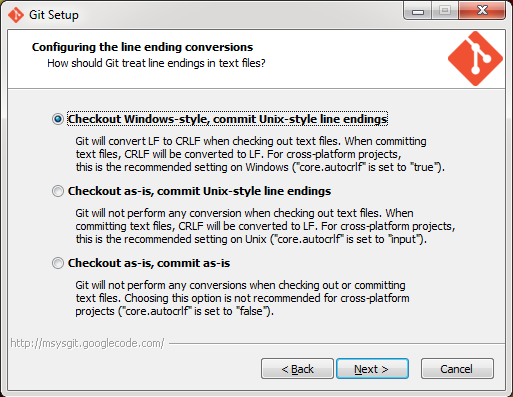
\includegraphics[width=.45\textwidth,keepaspectratio=true]{5.png} 
  \end{center} 
  \caption{Se acepta que se cambie automáticamente el cambio de línea} 
\end{figure} Esta opción de cambiar automáticamente el cambio de línea, permite que en Windows se trabaje normalmente con los archivos (manteniendo el indicador de cambio de línea de Windows) y que al hacer \textbf{commit} se cambie automáticamente este indicador al de Linux. Al realizar un \textbf{checkout}, Git convertirá los cambios de línea de Linux a Windows, para poder trabajar en ellos. Esto facilita la edición de código en ambos sistemas por parte de los desarrolladores. 
\clearpage
Una vez instalado, se tiene una versión de línea de comandos (incluyendo un cliente SSH que será muy útil para acceder a los servidores) y la interfaz gráfica de usuario estándar. 
\begin{figure}[hb] 
  \begin{center} 
    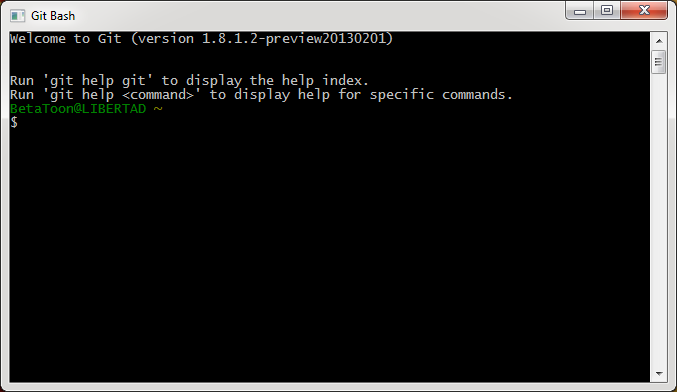
\includegraphics[width=.5\textwidth,keepaspectratio=true]{7.png} 
  \end{center} 
  \begin{center} 
    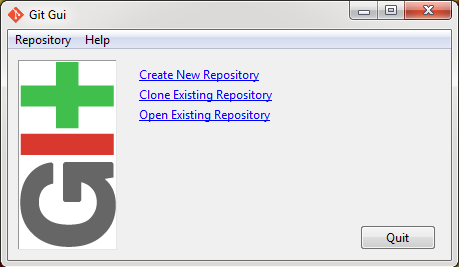
\includegraphics[width=.5\textwidth,keepaspectratio=true]{8.png} 
  \end{center} 
\end{figure} Nota sobre el uso en Windows: se usar, siempre que sea posible, Git con el shell que se instala (estilo Unix), que permite utilizar las complejas líneas de comando que figuran en este documento. Si usted necesita, por alguna razón, utilizar la interfaz de comandos nativa de Windows, se deben tener otras consideraciones para hacerlo, para esto consulte la documentación de Git (\url{http://www.git-scm.co m/doc}).

\clearpage

\section{Configuración inicial} 
\label{sec:initialsetup} 
\subsection{Identidad} 
\label{sec:youridentity} Los primeros pasos a realizar, es adicionar nuestros datos personales a Git; a partir de aquí, se incluirán en cada cambio que realicemos. Una información importante aquí, es que Git hace distinción, como se verá más adelante, entre los que adicionan cambios al Git y los que realizaron los cambios\footnote{por ejemplo, si se está aplicando un flujo de trabajo con gerente integrador y la persona 
  \textbf{A} realiza un cambio realiza commit en su Git, luego envía el commit al integrador ( persona 
  \textbf{B}), el integrador revisa el commit y lo adiciona al servidor Git principal, para el servidor principal Git, el cambio lo realizó la persona 
  \textbf{A}, pero lo adicionó el integrador, manteniéndose la compartimentación en los cambios}. Esto se realiza de esta forma: 
\shellcmd{git config $--$global user.name ``John Doe''} 
\shellcmd{git config $--$global user.email johndoe@example.com} La opción ``\emph{$--$global}'' especifica que estas configuraciones serán globales, las predeterminadas. Si se desea que un proyecto tenga otra identidad, solo habría que omitir este parámetro y ejecutar los comandos 
\emph{dentro} del directorio d e trabajo. 
\chapter{Personalizando Git} 
\label{chap:customizinggit} 
\section{Configuración de Git} 
\label{sec:configuringgit} 
\subsection{Configuración básica del cliente Git} 
\label{sec:basicconf} 
\subsection{Colores en Git} 
\label{sec:colors} 
\subsection{Herramientas externas para fusionar y para comparar} 
\label{sec:externaltools} 
\subsection{Formato y espacios en blanco} 
\label{sec:formatsandspaces} 
\subsection{Configuración de Servidor} 
\label{sec:serverconf} 
\section{Atributos de Git} 
\label{sec:attributesgit} 
\subsection{Archivos binarios} 
\label{sec:binaryfiles} 
\subsubsection{Identificando archivos binarios} 
\label{sec:identifyingbinary} 
\subsubsection{Comparando archivos binarios} 
\label{sec:comparingbinaries}

\subsubsection{Expansión de palabras clave} 
\label{sec:expandingkeywords} 
\subsubsection{Exportación del repositorio} 
\label{sec:exportgit} 
\subsubsection{Estrategias de fusión} 
\label{sec:mergestrategies} 
\section{Puntos de enganche Git} 
\label{sec:hooks} 
\section{Un ejemplo de implantación de una determinada política en Git} 
\label{sec:policy} 
\subsection{Punto de enganche en el lado servidor} 
\label{sec:serverhook} 
\subsubsection{Obligando a utilizar un formato específico en el mensaje de confirmación de cambios} 
\label{sec:mandatorycommitmessage} 
\subsubsection{Implementando un sistema de control de accesos basado en usuario} 
\label{sec:userbasedaccesscontrol} 
\subsubsection{Obligando a realizar envíos solo-de-avance-rápido (Fast-Forward-Only pushes)} 
\label{sec:onlyfastforward} 
\subsection{Puntos de enganche del lado cliente} 
\label{sec:clienthook}


\chapter{Git y Subversion} 
\label{chap:gitsvn} 
\section{Utilizando Git como cliente para servidor Subversion} 
\label{sec:gitclientsvn} Debido a su diseño modular, Git puede integrarse con otros 
\gls{scv}. Este nivel d e integración permite tanto importar proyectos, como trabajar como cliente de otro s 
\gls{scv}. En el caso de Subversion, esto se realiza por medio del parámetro 
\textbf{svn} adicionado al comando 
\textbf{git}, de esta forma: 
\shellcmd{git svn} Para acceder a la ayuda y ver los comandos que se pueden utilizar, se puede ejecutar: 
\shellcmd{git help svn} 
\subsection{Haciendo svn checkout} 
\label{sec:svncheckout} Si el repositorio Subversion ubicado en 
\emph{URL} cumple con el estándar de crear carpetas para desarrollo, versiones y ramas de desarrollo (trunk, tags y branch es), se ejecuta:
\shellcmd{git svn clone -s 
  \emph{URL}} Esto crea automáticamente las ramas y los tags en Git, según estén definidos en el subversion. Para especificar el nombre de los directorios, en caso de que no coincidan con l os nombres en inglés, sería ejecutar esta variación del comando, especificando los nombres reales: 
\shellcmd{git svn clone 
  \emph{URL} -T trunk -b branches -t tags} A partir de aquí se puede continuar el desarrollo utilizando Git y luego sincronizando los cambios con el Subversion, como por ejemplo, de esta forma: 
\begin{enumerate} 
\item Crear una rama propia, para desarrollo: 
  \shellcmd{git checkout -b work trunk} 
\item Modificar y adicionar cambios al repositorio, utilizando ``git add'' y ``git commit'' según se desee. 
\item Sincronizar con el servidor de subversion remoto utilizando 
  \shellcmd{git svn dcommit} 
\end{enumerate} Llegados a este punto, conviene brindar algunas recomendaciones: 
\begin{enumerate} 
\item 
\end{enumerate} 
\section{Comandos Subversion y equivalentes en Git} 
\label{sec:git2svn} Pasamos a ver los comandos más utilizados en Subversion y cómo se realizaría esa tarea utilizando Git:

\subsection{Crear repositorio} 
\label{sec:createsvnrepo} 
\begin{tabular}{| l | l |} 
  \hline subversion: & git: \\
\hline 
  \colorbox{mygray}{\texttt{\textbf{\footnotesize\$} svnadmin create repo}} & \colorbox{mygray}{\texttt{\textbf{\footnotesize\$} git init}} \\
\hline 
  \colorbox{mygray}{\texttt{\textbf{\footnotesize\$} svn import \emph{URL}}} & \colorbox{mygray}{\texttt{\textbf{\footnotesize\$} git add .}}  \\
\hline & \colorbox{mygray}{\texttt{\textbf{\footnotesize\$} git commit}}\\
\hline 
\end{tabular}% 
\begin{description} 
\item [git init] inicializa el repositorio local, creando el directorio 
  \textbf{ .git}. 
\item [git add .] adiciona a git todo el contenido del directorio. 
\item [git commit] adiciona los cambios al historial de Git. 
\end{description} 
\subsection{Creando la copia de trabajo}\label{sec:svnworkdir} Para crear la copia o directorio de trabajo, se ejecuta: 
\svngit{svn checkout 
  \emph{URL}}{git clone 
  \emph{URL}} A diferencia del comando ``svn checkout'', el de Git descarga TODO el historial del directorio subversion. Si el directorio ubicado en esa dirección cumple 
\subsection{Adicionando cambios} 
\label{sec:commit} 
\begin{tabular}{| l | l |} 
  \hline subversion: & git: \\
\hline 
  \colorbox{mygray}{\texttt{\textbf{\footnotesize\$} svn commit}} & \colorbox{mygray}{\texttt{\textbf{\footnotesize\$} git commit -a }} \\
\hline 
\end{tabular}

% Aquí hay que aclarar algunas cosas: 
\begin{itemize} 
\item Como se ha dicho anteriormente, el ``git commit'' 
\end{itemize} 
\begin{tabular}{| l | l |} 
  \hline subversion: & git: \\
\hline 
  \colorbox{mygray}{\texttt{\textbf{\footnotesize\$} svnadmin commit}} & \colorbox{mygray}{\texttt{\textbf{\footnotesize\$} git commit -a }}  \\
\hline 
\end{tabular}%

% 
\svngit{svn checkout \emph{URL}}{git clone \emph{URL}} 
\chapter{Otras operaciones con Git} 
\label{chap:othergit} 
\section{Buscar error en el código utilizando Git} 
\label{sec:testingwithgit} Git, con la ayuda del comando ``\emph{bisect}'' permite buscar por búsqueda binaria el cambio que introdujo un error. Este comando usa 
\emph{git rev-list $--$bisect} para ayudar al proceso de búsqueda binaria a encontrar el cambio que introdujo un error, a partir de un 
\textbf{commit} declarado como ``bueno'', donde no existía ese error y uno ``malo'' donde se confirmó que existía. Este proceso se puede automatizar de la siguiente forma: 
\begin{enumerate} 
\item Crear una prueba, como un script a ejecutar. Este script debe cumplir algunos requisitos: 
  \begin{itemize} 
  \item Deberá salir con código 0 si el código fuente actual es bueno, no contiene errores.
  \item Termina con un código entre 1 y 127 (incluyendo 127), excepto 125, si el código fuente actual es defectuoso. 
  \end{itemize} 
\end{enumerate} 
\begin{verbatim}
$ cat ~/test.sh 
  #!/bin/sh make || exit 125
  ~/check_test_case.sh
$ git bisect start HEAD HEAD~10 - # evita los commits que no compilan
$ git bisect run ~/test.sh   # ejecuta el script de verifica el error
\end{verbatim}


Al ejecutar: \emph{git bisect start HEAD HEAD\~{}10 $--$} se especifica que \emph {HEAD}\footnote{identifica al último commit realizado a la rama} es una revisión con el error y que 10 revisiones antes no lo había (\emph{HEAD\~{}10})

\glsaddall 
\printglossaries 
\end{document}

